\section{Running Example: The Cinderella-Stepmother Game}
\label{sec:example}

For the purposes of this paper, we will illustrate how the validity
guided-synthesis algorithm works, using a variation of the minimum-backlog
problem, the two player game between Cinderella and her wicked
Stepmother, first  expressed by Bodlaender \textit{et
al.}~\cite{bodlaender2012cinderella}.

The main objective for Cinderella (i.e. the reactive system) is to prevent a
collection of buckets from overflowing with water. On the other hand,
Cinderella's Stepmother (i.e. the system's environment) refills the buckets with a predefined amount of water that is distributed in a random fashion between the buckets.
For the running example, we chose an instance of the game that has been
previously used in template-based synthesis~\cite{beyene2014constraint}. In this instance, the game is described
using five buckets, where each bucket can contain up to two units of water.
Cinderella has the option to empty two adjacent buckets at each of her turns,
while the Stepmother distributes one unit of water over all five buckets. In the context of this paper we use this example to show how specification is expressed, as well as how we can synthesize an efficient implementation that describes reactions for Cinderella, such that a bucket overflow is always prevented.



\section{Background}
\label{sec:background}

\begin{figure}[!t]
\centering
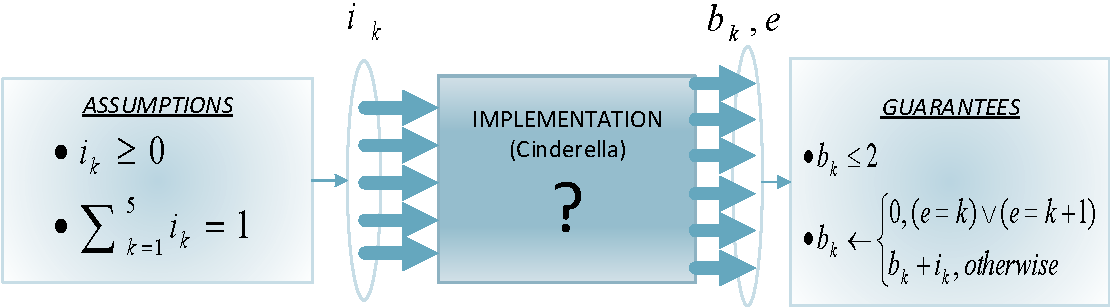
\includegraphics[scale=0.55]{agcontracttilted-crop.pdf}
\caption{An Assume-Guarantee Contract.}
\label{fg:agcontract}
\end{figure}

\iffalse
In this section we define Assume-Guarantee contracts (Section~\ref{sec:pre}),
describe the problem of synthesis in terms of discovering inductive invariants that imply the realizability of the given specification (Section~\ref{sec:formals}), and give a background on our main solving engine (Section~\ref{sec:aeval}).
%Finally, we enrich our formal definitions with an informal proof of the
%algorithm's correctness in terms of the successfully synthesized
%implementations.

\subsection{Assume-Guarantee Contracts}
\label{sec:pre}
\fi

We focus our interest on a mainstream variation for representing system requirements, using an \textit{Assume-Guarantee
Contract}. Requirements in this format contain two main types of constraints.
The \emph{assumptions} of the contract restrict the possible inputs that the
environment can provide to the system, while the \emph{guarantees} are used to
describe what is considered a safe reaction of the system to the outside world.

A (conceptually) simple example is shown in Figure~\ref{fg:agcontract}. The contract describes a possible set of requirements for a specific instance of the Cinderella-Stepmother game that we introduced in Section~\ref{sec:example}. Our goal is to synthesize an implementation that describes Cinderella's winning region of the game. Cinderella in this case is the implementation, as shown by the middle box in Figure~\ref{fg:agcontract}. Cinderella's inputs are five different values $i_k, 1 \leq k \leq 5$, determined by a random distribution of one unit of water by the Stepmother. During each of her turns Cinderella has to make a choice denoted by the output variable $e$, such that the buckets $b_k$ do not overflow during the next action of her Stepmother. We define the contract using the set of assumptions $A = \{i_k \geq 0, \sum_{k=1}^{5} i_k = 1\}$ and the guarantees $G = \{b_k \leq 2, b_k = ite((e=k \lor e=k+1), 0, (b_k+i_k))\}$. For the particular example, it is possible to construct at least one implementation that satisfies the guarantee constraints, given the input assumptions. The proof of existence of such an implementation  is the main concept behind the \emph{realizability} problem, while the automated construction of a witness implementation is the main focus of \emph{program synthesis}.


Since the contract in Figure~\ref{fg:agcontract} is \emph{realizable}, an efficient synthesis procedure would be capable of providing at least one
implementation. At this point it is important to consider a variation of the example, where $A = \varnothing$. This is a practical case of an
\emph{unrealizable} contract, as there is no feasible Cinderella implementation that can correctly react to Stepmother's actions. The most apparent counterexample in this case is that the Stepmother is able to pour random amounts of water, and would be capable to overflow at least one bucket during every one of her turns.

\subsection{Formal Representation}
\label{sec:formals}
We use two disjoint sets, $state$ and $inputs$, to describe a system.
A straightforward and intuitive way to represent an \emph{implementation} is by
defining a \emph{transition system}, composed of an initial state
predicate $I(s)$ of type $state \to bool$, as well as a transition relation
$T(s,i,s')$ of type $state \to inputs \to state \to bool$.

Combining the above, we represent an Assume-Guarantee (AG) contract using a set
of \emph{assumptions}, $A: state \rightarrow inputs \rightarrow bool$,
and a set of \emph{guarantees} $G$. The latter is further decomposed into two
distinct subsets $G_I: state \rightarrow bool$ and $G_T: state \rightarrow
inputs \rightarrow state \rightarrow bool$. $G_I$ defines the set of valid
initial states, and $G_T$ contains constraints that need to be satisfied in
every transition between two states. An important note at this point is that we
do not make any distinction between internal state variables and outputs in the
formalism. This alone allows us to use state variables to (in some cases)
simplify the specification of guarantees, since we do not expect a contract
to be always defined over all variables in the transition system.

Consequently, we can formally define a realizable contract, as one for which any
preceeding state $s$ can take a transition into a new state $s'$ that satisfies
the guarantees, assuming valid inputs. For a system to be ever-reactive, these
new states $s'$ should be further usable as preceeding states in a future
transition. States like $s$ and $s'$ are defined as being \textit{viable}, if
and only if:
\begin{align}
\begin{split}
  \viable(s) &=
  \forall s,i. (A(s, i) \Rightarrow \exists s'.~ G_T(s, i,s')
\land \viable(s')).
\label{eq:viable}
\end{split}
\end{align}
This equation is recursive and we interpret it coinductively, i.e., as a
greatest fixed-point.
A necessary condition, finally, is that the set of viable states
intersects with the set of initial states. As such, to conclude that a contract
is realizable, we require that
\begin{equation}
\exists s. G_I(s) \land \viable(s).
\label{eq:nonempty}
\end{equation}

The intuition behind our proposed algorithm in this paper relies on the
discovery of a greatest fixpoint that only contains viable states. In the case where a fixpoint is computed, we proceed by extracting a witnessing collection of reactions that are, by construction, guaranteed to satisfy the specification. To achieve both the fixpoint generation, as well as the witness extraction, we depend on \aeval, a solver for $\forall\exists$-formulas.

\subsection{\textit{AE-VAL}}
\label{sec:aeval}

\begin{figure}[!t]
\centering
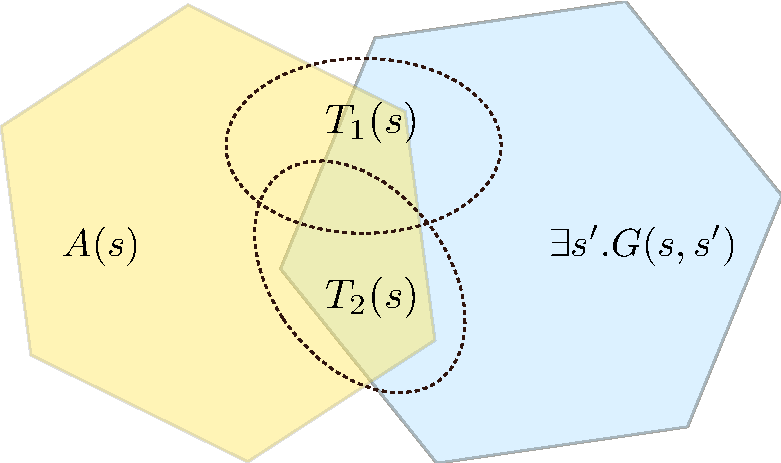
\includegraphics[width=2.5in]{aeval_invalid}
\caption{Region of validity computed for an example requiring \aeval to iterate two times.}
\label{fg:aeval}
\end{figure}

\aeval~\cite{fedyukovich2015automated} is an algorithm to decide validity and extract Skolem functions.
It takes as input a formula of the form $\forall s \,.\,  A(s) \Rightarrow \exists s' . G(s,s')$, 
where $A(s)$ has only existential\andreas{you meant universal here, right?} quantifiers, and $G(s,s')$ is quantifier-free.
%
While deciding the validity, \aeval iteratively enumerates models of $A(s) \land G (s, s')$ and groups them into a set of partitions $\{P_i(s)\}$, such that each $P_i(s) \Rightarrow \exists s' . G (s, s')$.
We say that after $n$ iterations, \aeval establishes a formula $R_n(s) \eqdef \bigvee_{i=1}^n P_i(s)$ which is by definition an under-approximation of $\exists s' . G (s, s')$.

If after $n$ iterations, it happens that $A(s) \Rightarrow R_n(s)$ then $\forall s \,.\,  A(s) \Rightarrow \exists s' . G(s,s')$ is valid, and \aeval generates a Skolem function as described in~\cite{katis2016synthesis}.
Alternatively, if $A(s) \land  G (s, s') \land \neg{R_n (s, s')}$ is unsatisfiable, then $A(s) \land \neg G (s, s')$ is satisfiable, or equivalently $\forall s \,.\,  A(s) \Rightarrow \exists s' . G(s,s')$ is invalid (see an example in Figure~\ref{fg:aeval}).
In both cases, we say that $A(s) \land R_n(s)$ is a \emph{region of validity}, meaning that $\forall s \,.\,  A(s) \land R_n(s) \Rightarrow \exists s' . G(s,s')$ is valid by construction.

\begin{lemma}
If formula $\forall s \,.\,  A(s) \Rightarrow \exists s' . G(s,s')$ is invalid, and $A(s) \land R_n(s)$ is the region of validity, then there is no other formula $S(s)$ such that $A(s) \land R_n(s) \Rightarrow S(s)$ and $\forall s \,.\,  S(s) \Rightarrow \exists s' . G(s,s')$.

\label{lem:subset}
\end{lemma}

